\section{Color Transparency}
Color transparency (CT), a characteristic prediction of QCD, refers to the
reduction of initial and final state interactions between a hadron and the
nuclear medium in exclusive processes at large momentum transfer $Q^2$.
The concept was first independently proposed by Mueller and Brodsky in the
context of perturbative QCD, but was later shown to arise in nonperturbative
models.
% An analogue of CT can be seen in QED--a small $e^+e^-$ pair has a small cross
% section determined by its dipole moment.


The three requirements for CT are the following:
\begin{itemize}
    \item Squeezing: the formation of a small configuration of quarks, sometimes
          referred to as a point-like configuration (PLC)
    \item This PLC is color-neutral outside its radius
    \item Freezing: the PLC maintains its small size over a distance comparable
          to or greater than the nuclear radius
\end{itemize}
There is theoretical support for selection of PLCs in exclusive processes.
Strength of interaction is proportional to transverse size of hadron interacting
with the nuclear medium.
Freezing time can be approximated and has been studied.
Moreover, CT is a necessary condition for the validity of QCD factorization
theorems.
ELABORATE AND SOFTEN THIS CLAIM.


% Previous experiments looking for the onset of CT have been suggestive of the
% meson electro/photoproduction
% $A(p,2p)$ at BNL
% $A(e,e'p)$ at SLAC and JLab


In experiments studying the color transparency phenomenon, a common observable
is the nuclear transparency.
It is generally of the form $T=\sigma_A/A\sigma_0$,
the ratio of
the per-nucleon cross section for some exclusive scattering process
to
the cross section for the same process on a free nucleon.
Previous experiments have used slightly different definitions of nuclear
transparency depending on the experiment's particulars.
Studies of $A(p,2p)$, quasielastic proton knockout using a proton beam,
at Brookhaven National Lab (BNL)~\cite{Carroll_1988, Mardor_1998, Leksanov_2001, Aclander_2004}
used the ratio of $\frac{d\sigma}{dt}$,
where $t$ is the four-momentum transfer squared.
Studies of $A(e,e'p)$, quasielastic electron scattering,
at MIT-Bates~\cite{Garino_1992},
SLAC~\cite{Makins_1994, ONeill_1995}
and Jefferson Lab (JLab)~\cite{Abbot_1998, Garrow_2002, Rohe_2005}
used the ratio of charge-normalized yields $Y$ measured in experiment
and from Monte Carlo simulation, $T=Y^{exp}/Y^{MC}$.
Studies of $A(e,e'\pi^+)$, pion electroproduction,
at JLab~\cite{Clasie_2007, Qian_2010}
used the super-ratio of the ratio of yields from experiment and simulation
for a nucleus with $A$ nucleons in the numerator and hydrogen in the
denominator,
$T= \big(Y^{exp}/Y^{MC}\big)_{A} / \big(Y^{exp}/Y^{MC}\big)_{H}$.


Traditional Glauber multiple scattering theory predicts that $T$ is constant as
$Q^2$ increases.
In this picture, the transparency should follow the same
energy dependence of the nucleon-nucleon scattering cross sections which,
as shown in Fig~\ref{fig:pdg_nucleon_nucleon_cross_section}.
are relatively constant between lab momenta of
\SI{1}{\giga\electronvolt} and \SI{1}{\tera\electronvolt}.
The reduction of initial/final state interactions predicted by CT results in an
increase in nuclear transparency with $Q^2$.
An illustration of this behavior is shown in Fig~\ref{fig:CT_toy_prediction}.

\begin{figure}[!h]
    \centering
    \begin{subfigure}[b]{1.0\textwidth}
        \centering
        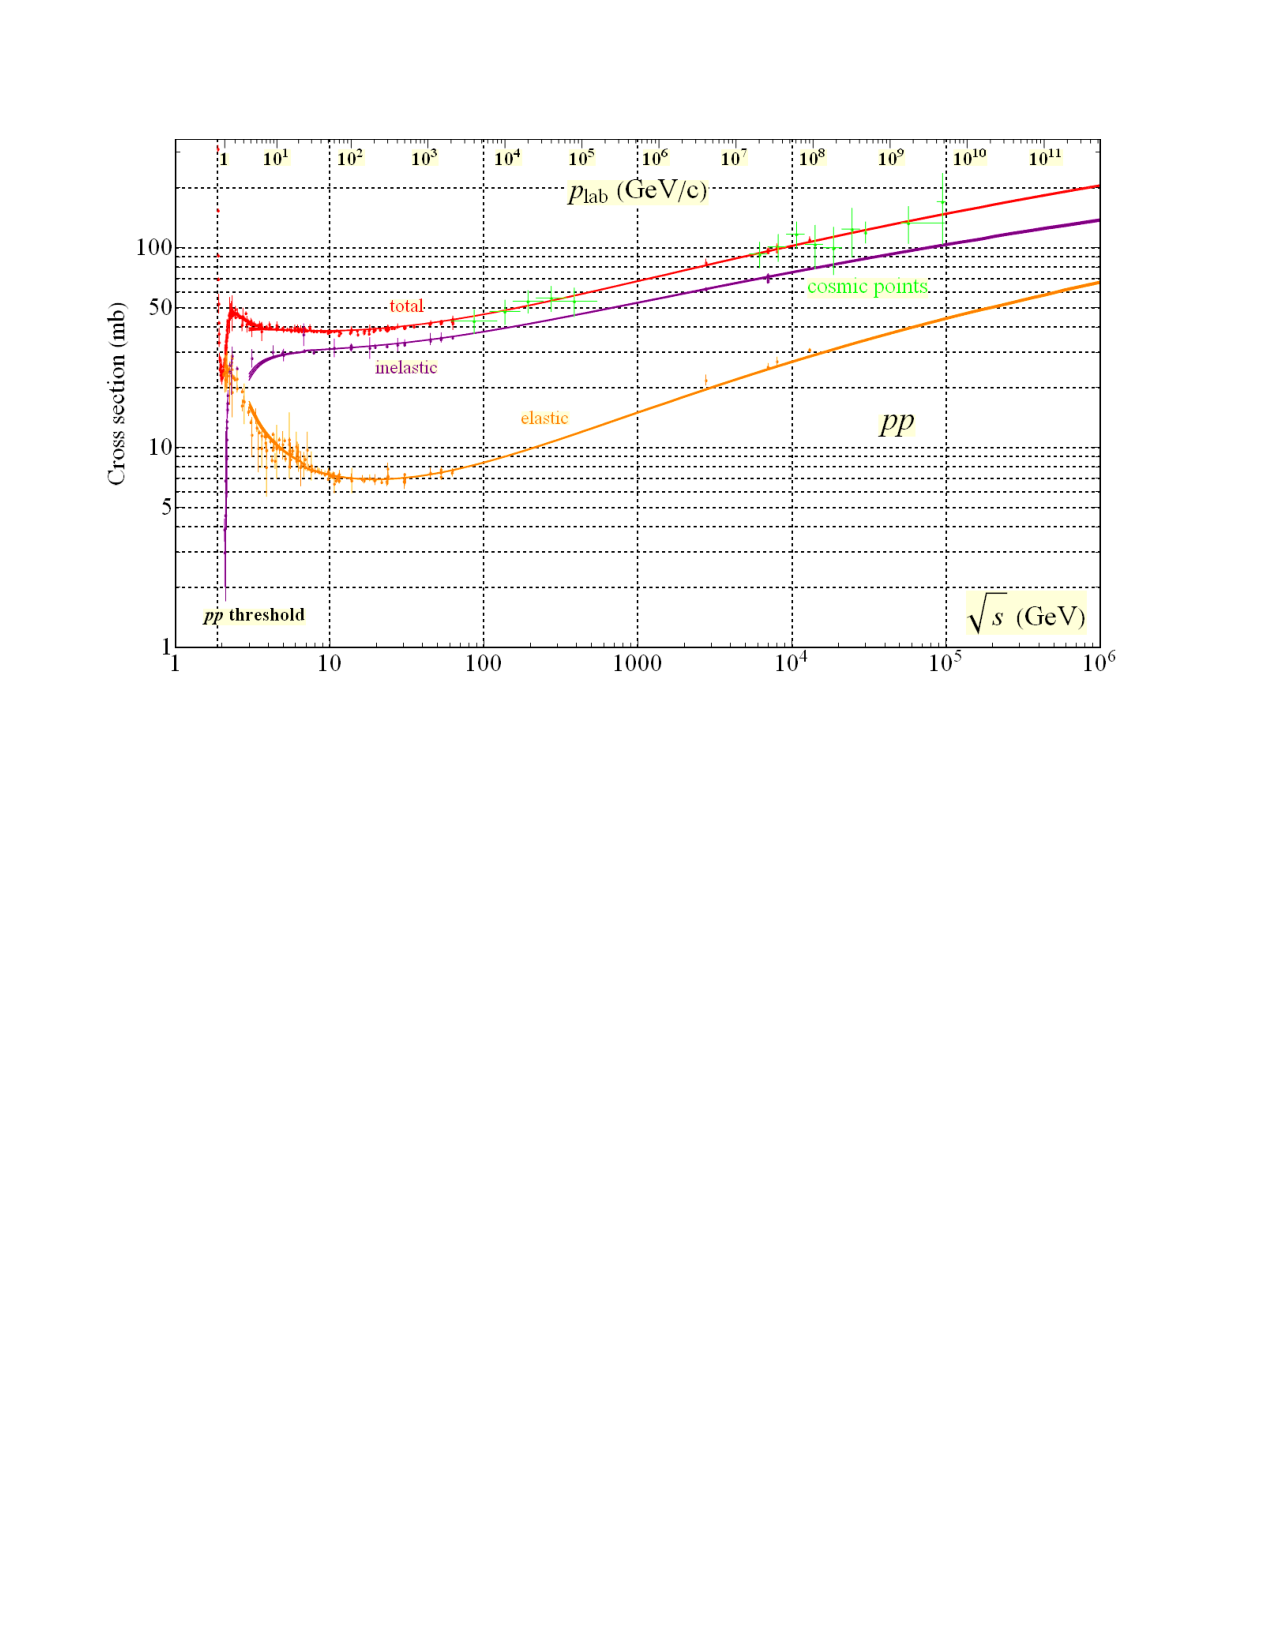
\includegraphics[width=1.0\textwidth]{chap2/pdg_pp_cross_section.pdf}
        \caption[Total, elastic, and inelastic $pp$ cross sections versus
                 $p_{lab}$ and $\sqrt{s}$.]{
                 Total, elastic, and inelastic $pp$ cross sections versus
                 $p_{lab}$ and $\sqrt{s}$.
                }
        \label{fig:pdg_pp_cross_section}
    \end{subfigure}
    \vspace{0.1cm}
    \\
    \begin{subfigure}[b]{1.0\textwidth}
        \centering
        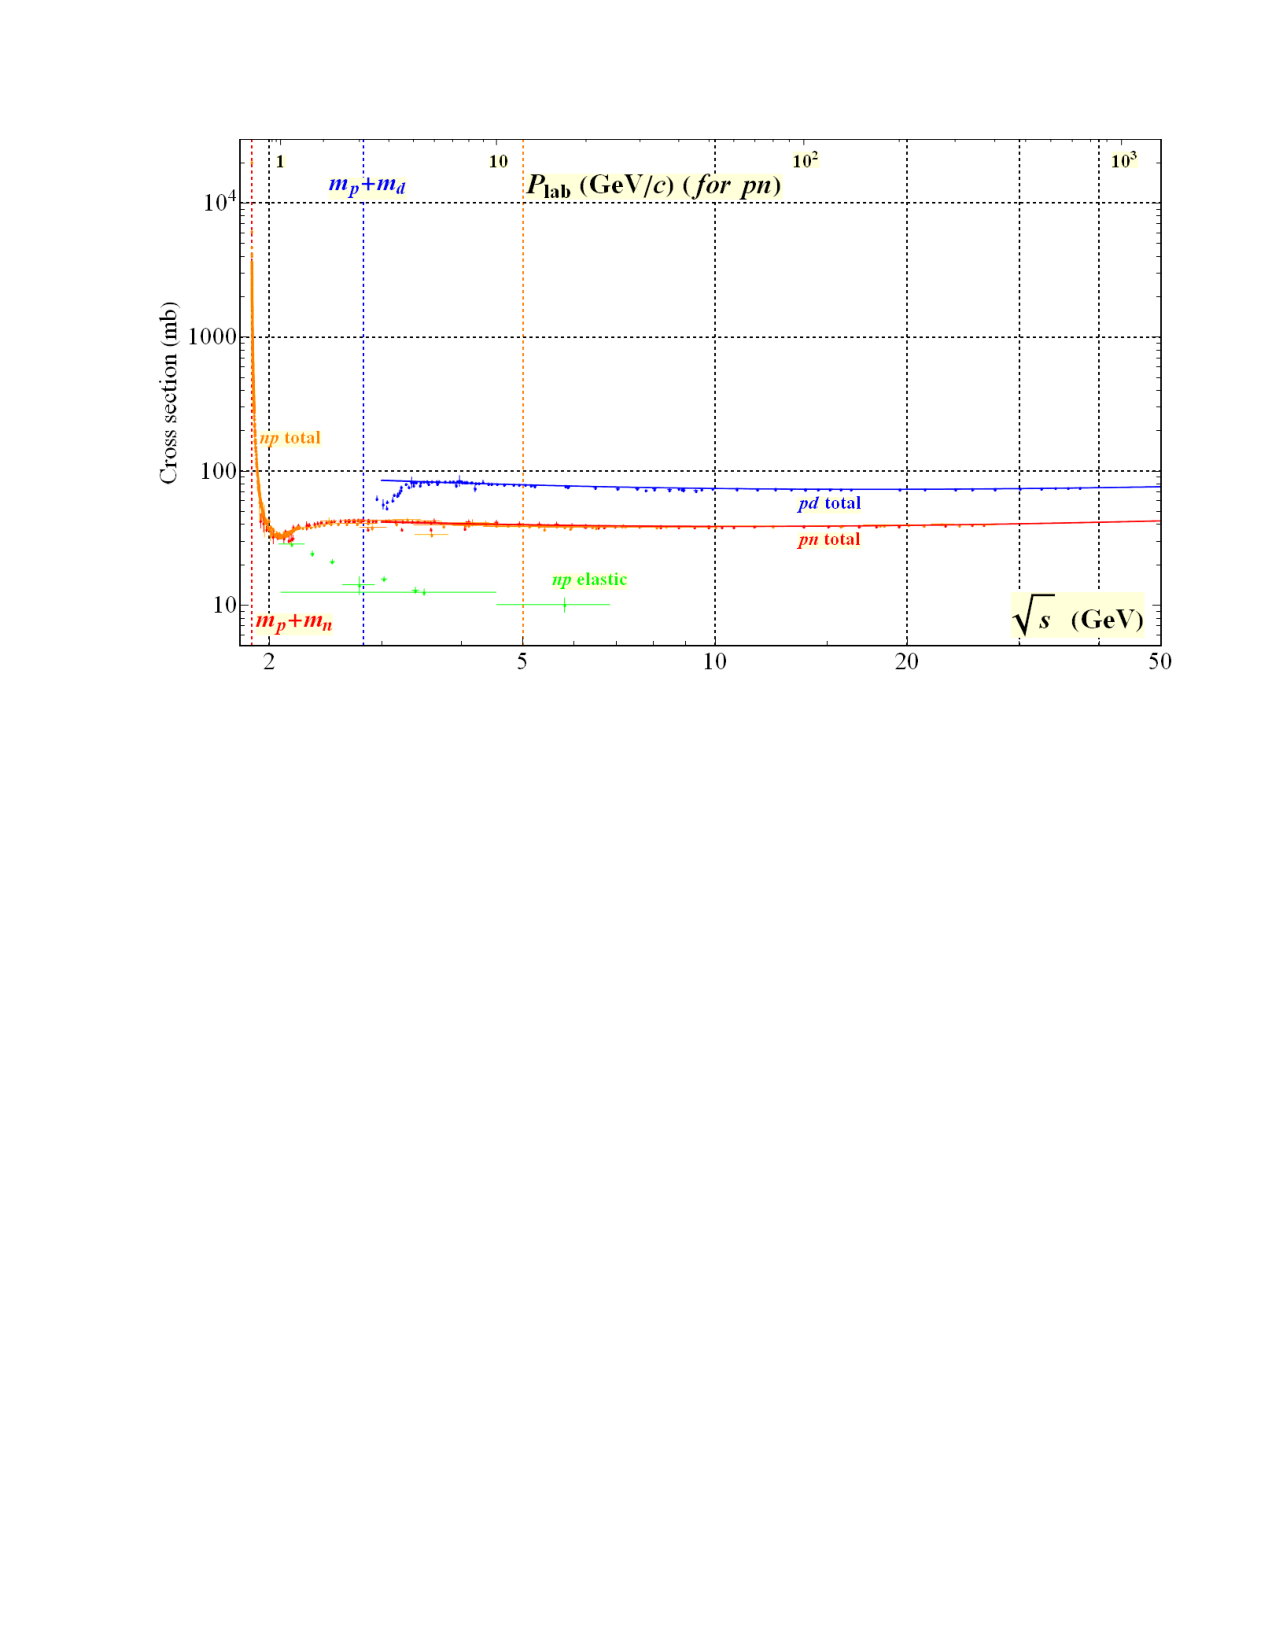
\includegraphics[width=1.0\textwidth]{chap2/pdg_pn_cross_section.pdf}
        \caption[Total $pn$ and $pd$ cross sections versus
                 $p_{lab}$ and $\sqrt{s}$.]{
                 Total $pn$ and $pd$ cross sections versus
                 $p_{lab}$ and $\sqrt{s}$.
                }
        \label{fig:pdg_pn_cross_section}
    \end{subfigure}
    \caption[Total, elastic, and inelastic $pp$, $pn$, and $pd$, cross sections
             versus lab momentum $p_{lab}$ and center of mass energy $\sqrt{s}$.]{
             Total, elastic, and inelastic $pp$, $pn$, and $pd$, cross sections
             versus lab momentum $p_{lab}$ and center of mass energy $\sqrt{s}$.
             Note that the total cross section is relatively constant over
             the range of momenta studied in E12-06-107, about
             \SIrange{4}{10}{\giga\electronvolt}.
             Figure reproduced from Ref~\cite{pdg_2020}.
             }
    \label{fig:pdg_nucleon_nucleon_cross_section}
\end{figure}


\begin{figure}[!h]
    \centering
    \includegraphics[width=0.8\textwidth]{chap1/CT_toy_prediction.pdf}
    \caption[ An illustration of the $Q^2$ dependence of nuclear transparency $T$
            for three scenarios.]{
            An illustration of the $Q^2$ dependence of nuclear transparency $T$
            for three scenarios.
            The blue line illustrates the prediction of the Glauber model,
            which has constant $T$ as $Q^2$ increases.
            The red line illustrates that for full color transparency, $T=1$;
            in this scenario there are no final state interactions between the
            ejected proton and the rest of the nucleus.
            The green line illustrates the scenario where the transparency
            begins to deviate from the Glauber prediction above an onset
            $Q_0^2$ and approach $T=1$ with increasing $Q^2$.
            }
    \label{fig:CT_toy_prediction}
\end{figure}
